\documentclass{article}
\usepackage{listings}
\usepackage{xcolor}
\usepackage{graphicx}
\usepackage{float}
\usepackage{hyperref}
\definecolor{codegreen}{rgb}{0,0.6,0}
\definecolor{codegray}{rgb}{0.5,0.5,0.5}
\definecolor{codepurple}{rgb}{0.58,0,0.82}
\definecolor{backcolour}{rgb}{0.95,0.95,0.92}

\lstdefinestyle{mystyle}{
    backgroundcolor=\color{backcolour},   
    commentstyle=\color{codegreen},
    keywordstyle=\color{magenta},
    numberstyle=\tiny\color{codegray},
    stringstyle=\color{codepurple},
    basicstyle=\ttfamily\footnotesize,
    breakatwhitespace=false,         
    breaklines=true,                 
    captionpos=b,                    
    keepspaces=true,                 
    numbers=left,                    
    numbersep=5pt,                  
    showspaces=false,                
    showstringspaces=false,
    showtabs=false,                  
    tabsize=2
}

\lstset{style=mystyle}

\title{The life and times of Michael K.}
\author{Mackenzie Norman}
\begin{document}
\maketitle
\begin{center}
    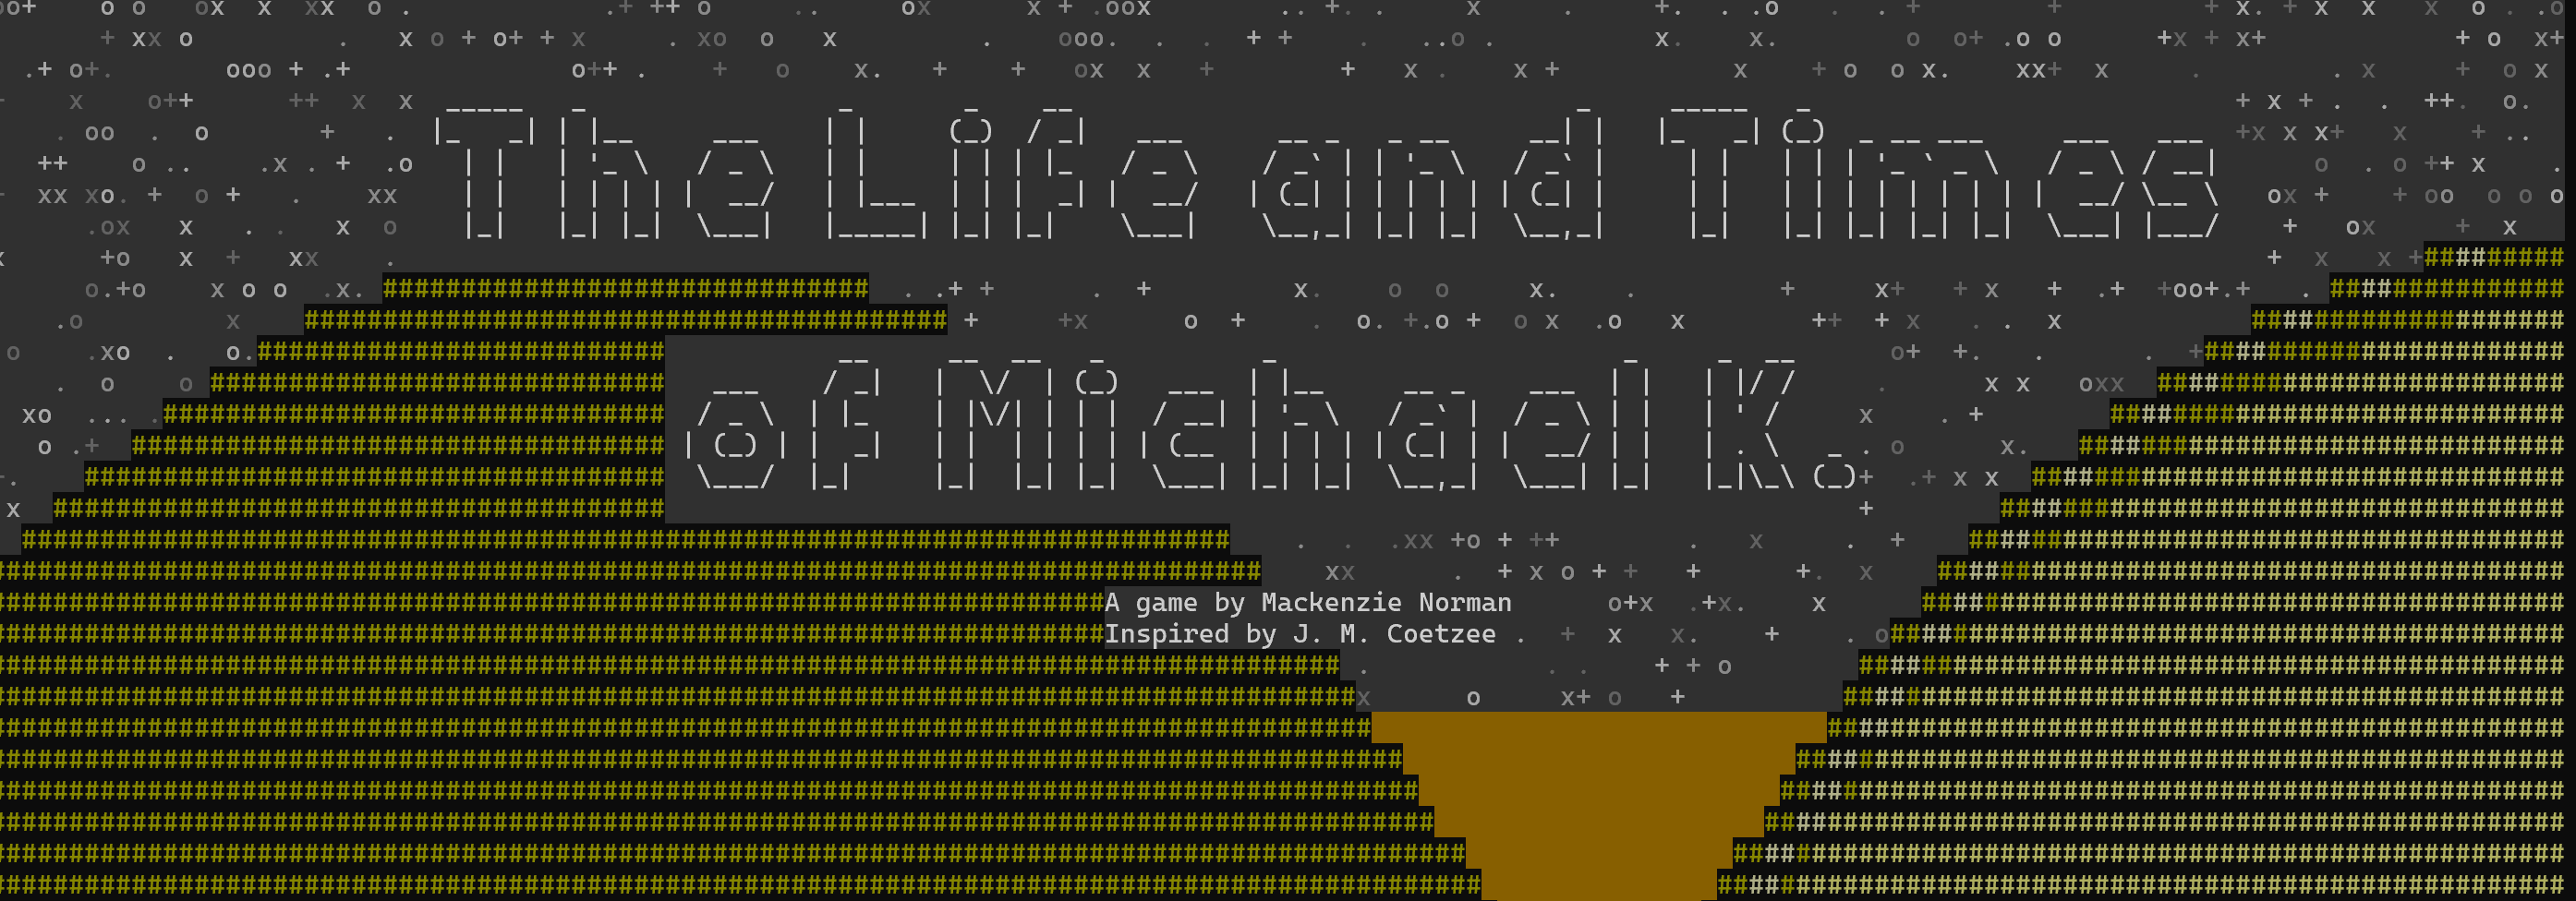
\includegraphics[width=\textwidth]{title_screen.png}
\end{center}
\section*{Instructions}
This game is designed in the style of other command line based games, and as such the graphics may not be beautiful, (although I they do require some creativity to get right). This means to run the program (properly) it you will need to access your command line.
If you struggle to run it you can also view the video I uploaded:  \url{https://youtu.be/MlMOhrKCtvw}
\paragraph{}

\subsection*{Installing}
Both versions (Mac \& Windows) have to downloaded from \url{https://github.com/mackenzie-norman/final-game/releases}
\subsubsection*{Mac}
I do not have a Mac so I have to rely in part of the kindness of my friend who compiled it for me but you will need to first open terminal \url{}

\subsubsection*{Windows}
This I can actually speak on. After downloading the file final-game.exe, go to your \textbf{Downloads} folder in explorer and click on the top and type ``\textbf{cmd}'' and press enter. 
\begin{figure}[H]
    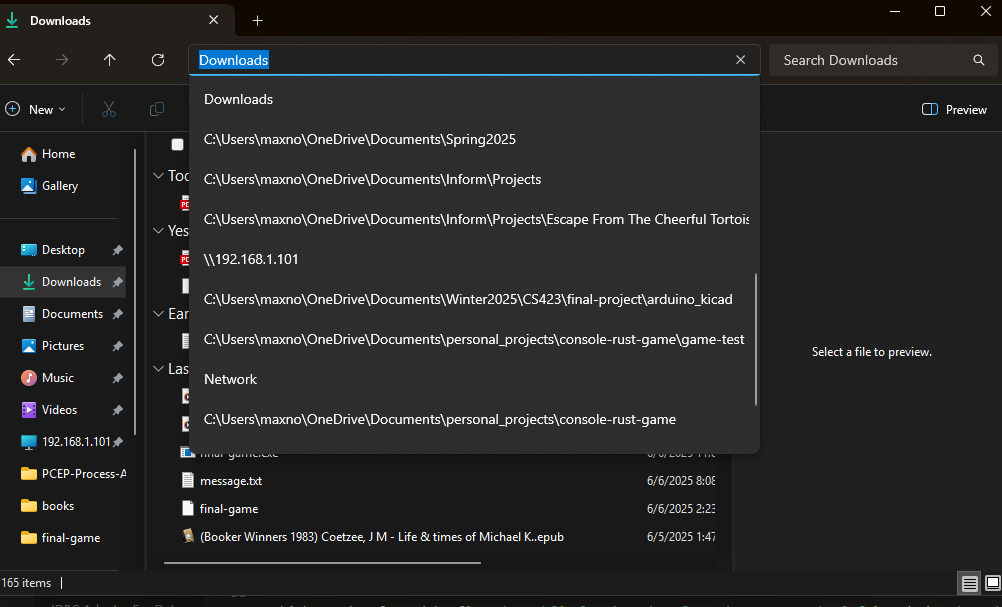
\includegraphics[width=\textwidth]{open-command-line.png}
    \caption{Opening the command line in windows}
        
\end{figure}

This should open the command line, expand it to full screen and type ``\textbf{.final-game.exe}'' and press enter. 
\begin{figure}[H]
    
\includegraphics[width=\textwidth]{fspic.png}
    \caption{A full screen command line with correct file entered}
        
\end{figure}

Windows might try to block it since it is unsigned but you should be able to open it up by clicking around it.


\subsection*{Gameplay}
The goal of the game (if you could call it that) is to garden. You begin the game with 10 pumpkin seeds and 2 Melon seeds.

Which can be planted by first \textbf{selecting them from the menu on the left} and then \textbf{clicking anywhere on the screen}

\textbf{Note:} You can always tell which menu option is selected because it will be highlighted in green.

    \begin{figure}[H]
    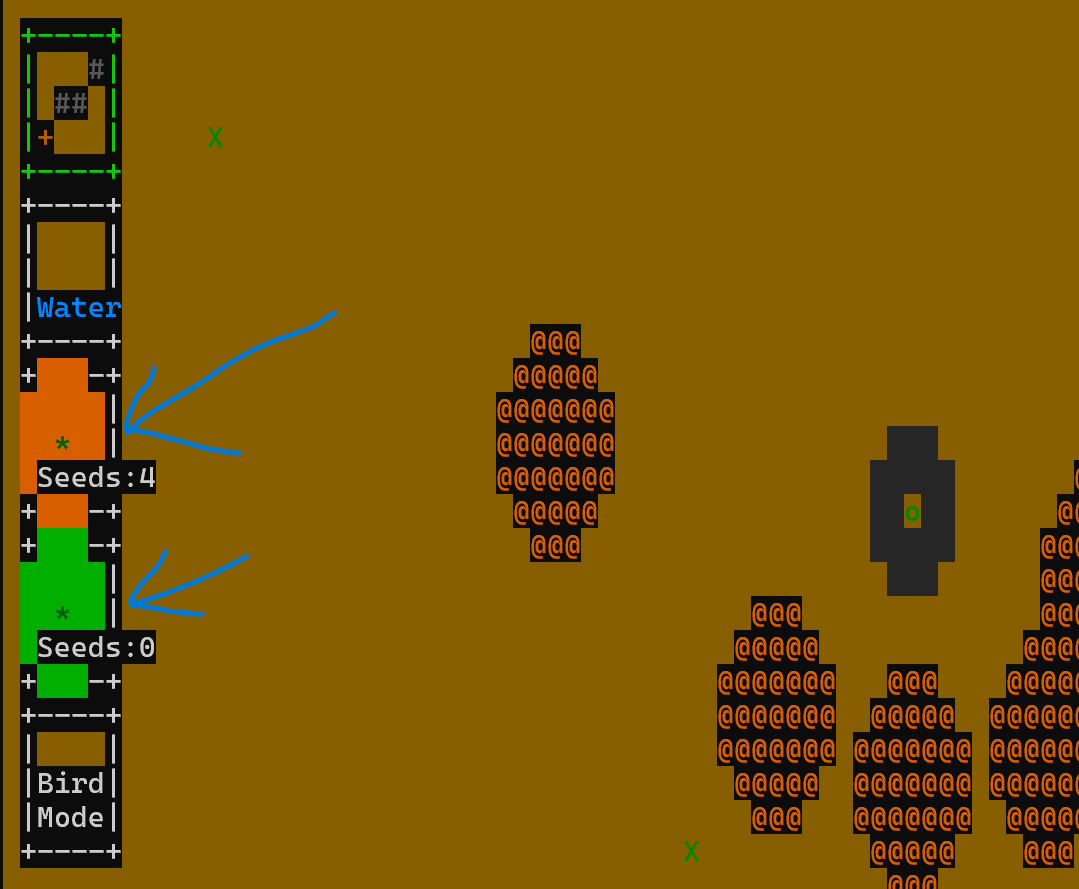
\includegraphics[width=\textwidth]{melons-pumpkins.png}
    \caption{Menu Option for Pumpkins and Melons}
        
    \end{figure}

Melons and Pumpkins cannot be planted on top of eachother, or on \textbf{weeds} which will grow randomly as the game progresses

The next thing you must do in order for your plants to grow is water them. You can do so by \textbf{selecting the water option from the menu on the left} which will allow you to click and water your plants. You can tell how well watered a plant is by the dark spot surrounding it. 

You water will run out as you water, to refill it, simply click the \textbf{pond} in the upper right corner, which will refill the water level.

    \begin{figure}[H]
    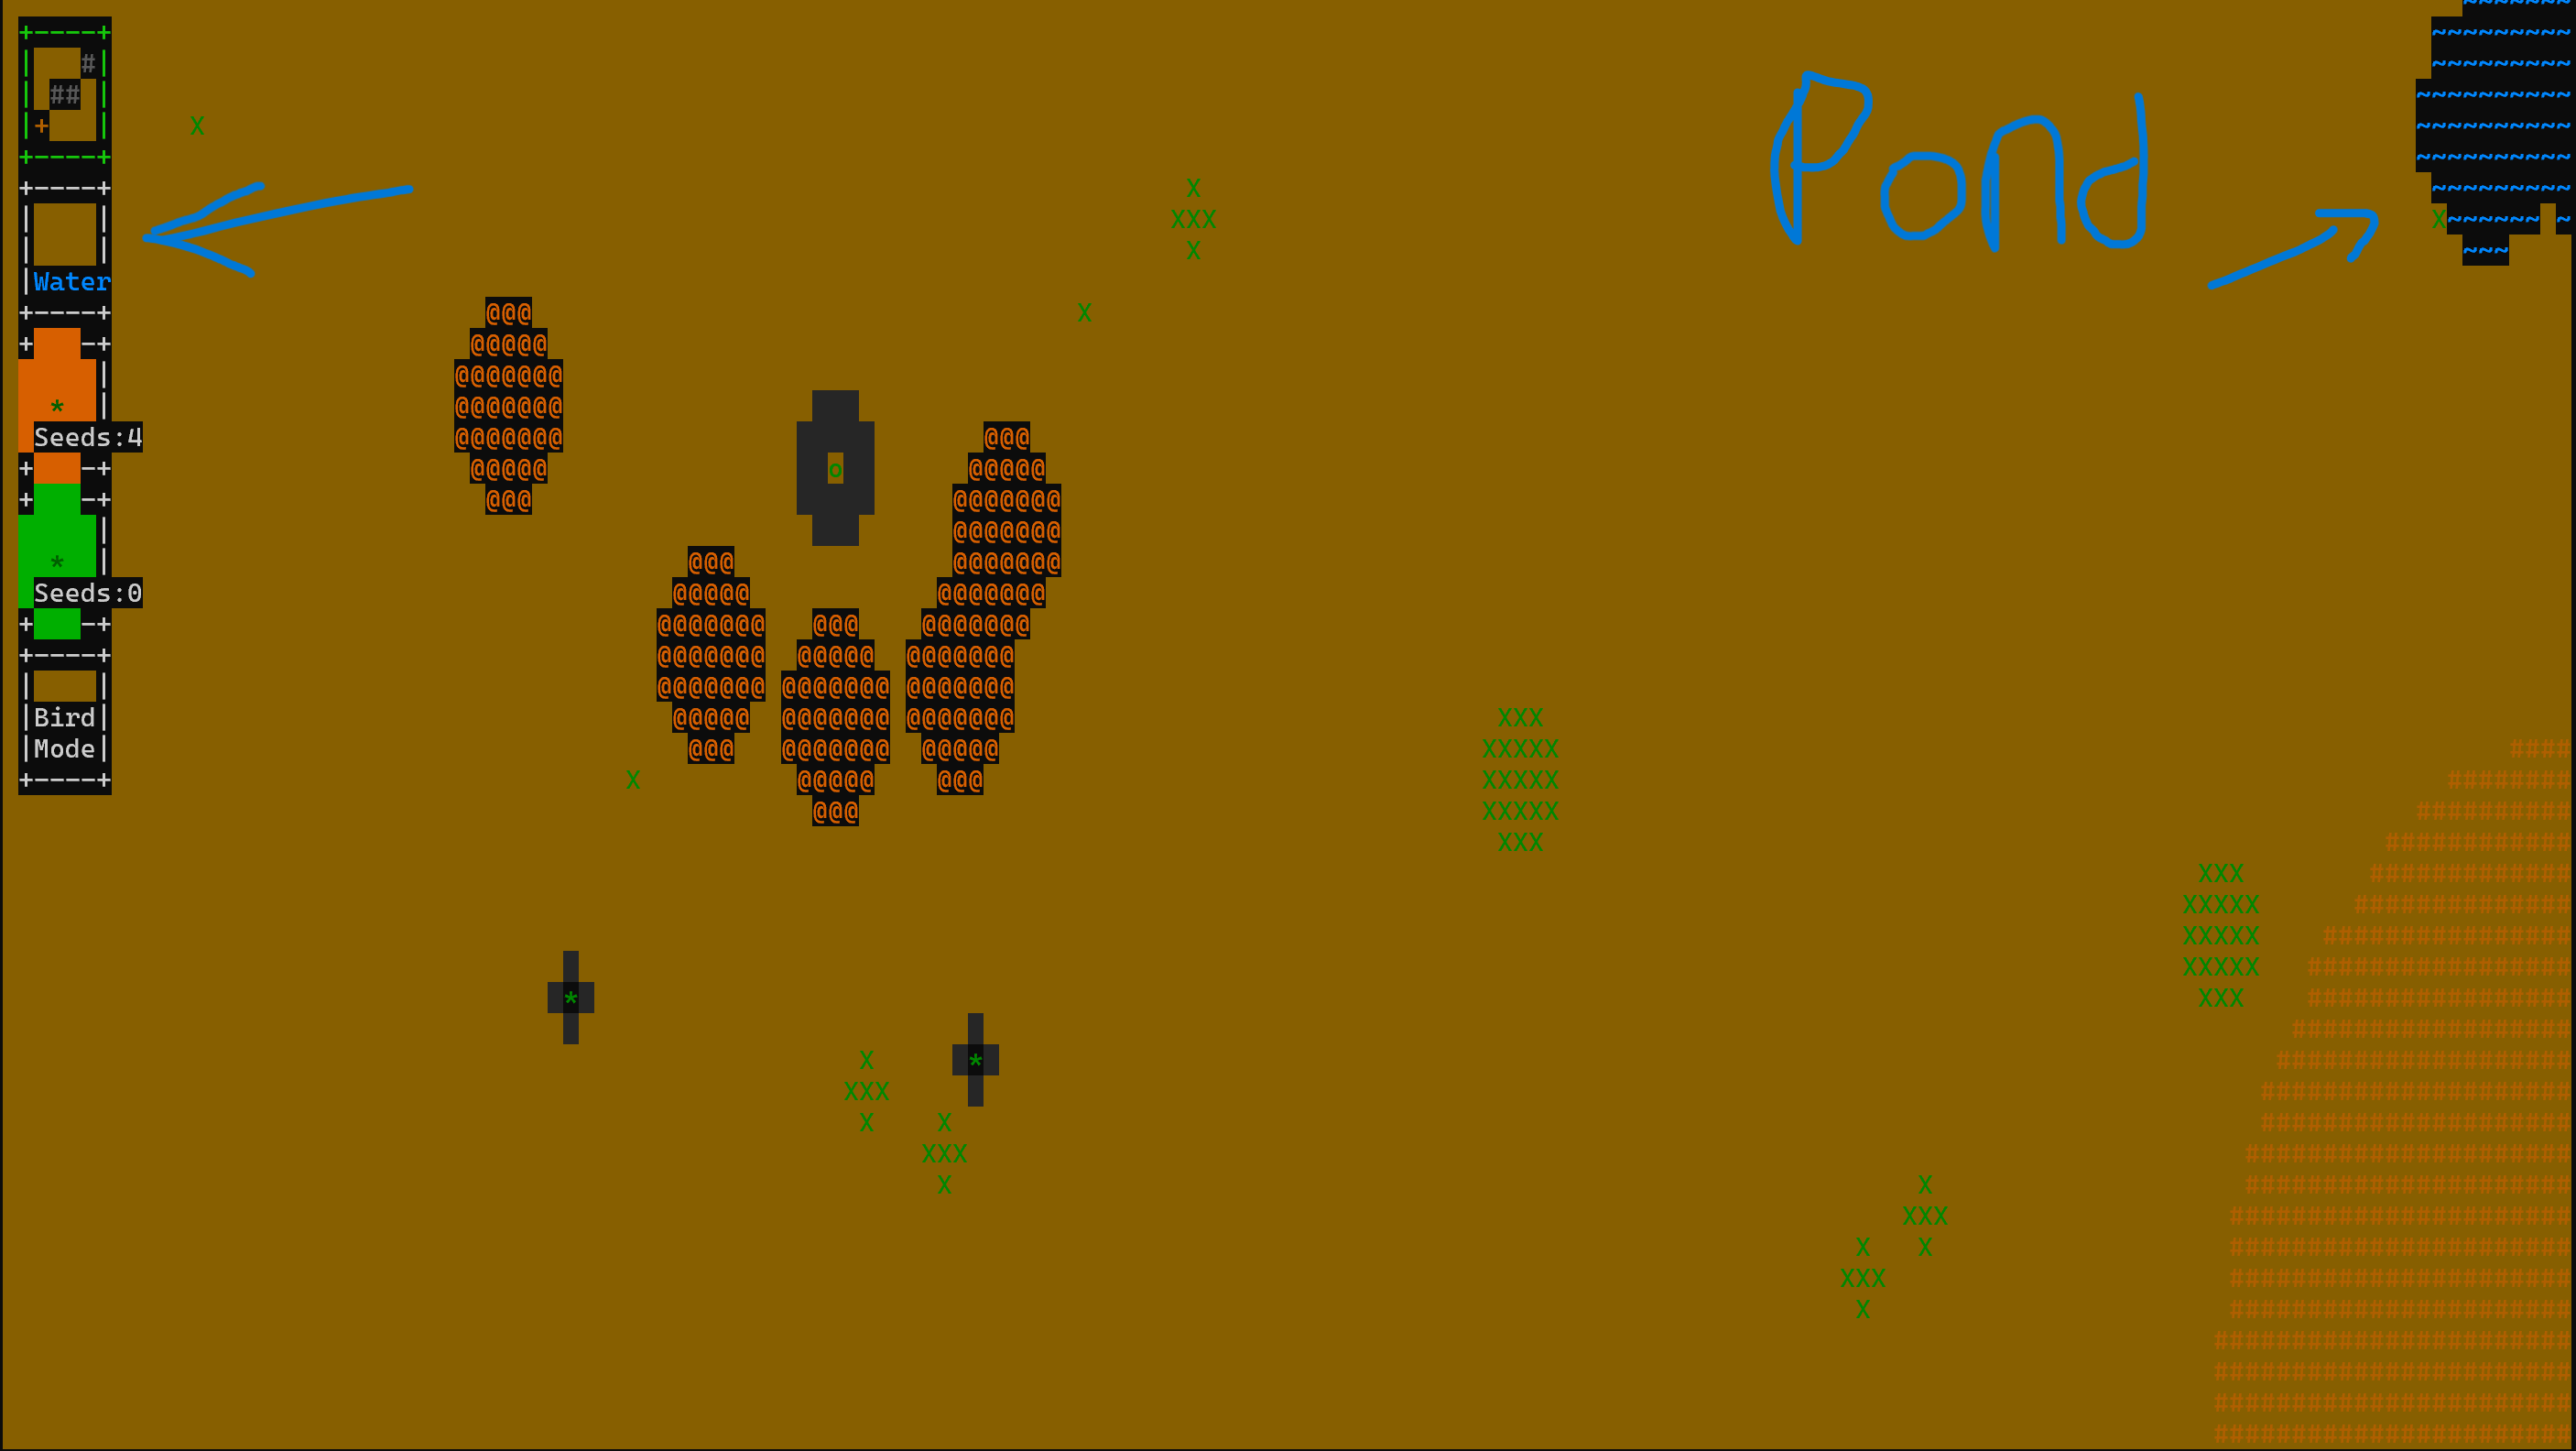
\includegraphics[width=\textwidth]{watering.png }
    \caption{Watering Instructions}
        
    \end{figure}

The first menu option is the hoe, this allows you to harvest Pumpkins and Melons for seeds by \textbf{clicking them}, and to remove weeds(if you want to, weeds aren't really harmful). Pumpkins and Melons can only be harvested when they are fully grown. It will take some time to learn what this looks like so be patient.

The final menu option is \textbf{Bird Mode} clicking this will take to a view where you are overlooking your garden from the perspective of a bird. While in this mode you cannot interact with your crops, but they will continue to grow (as will weeds).

To leave this mode, \textbf{click the large green arrow in the upper left}
    \begin{figure}[H]
    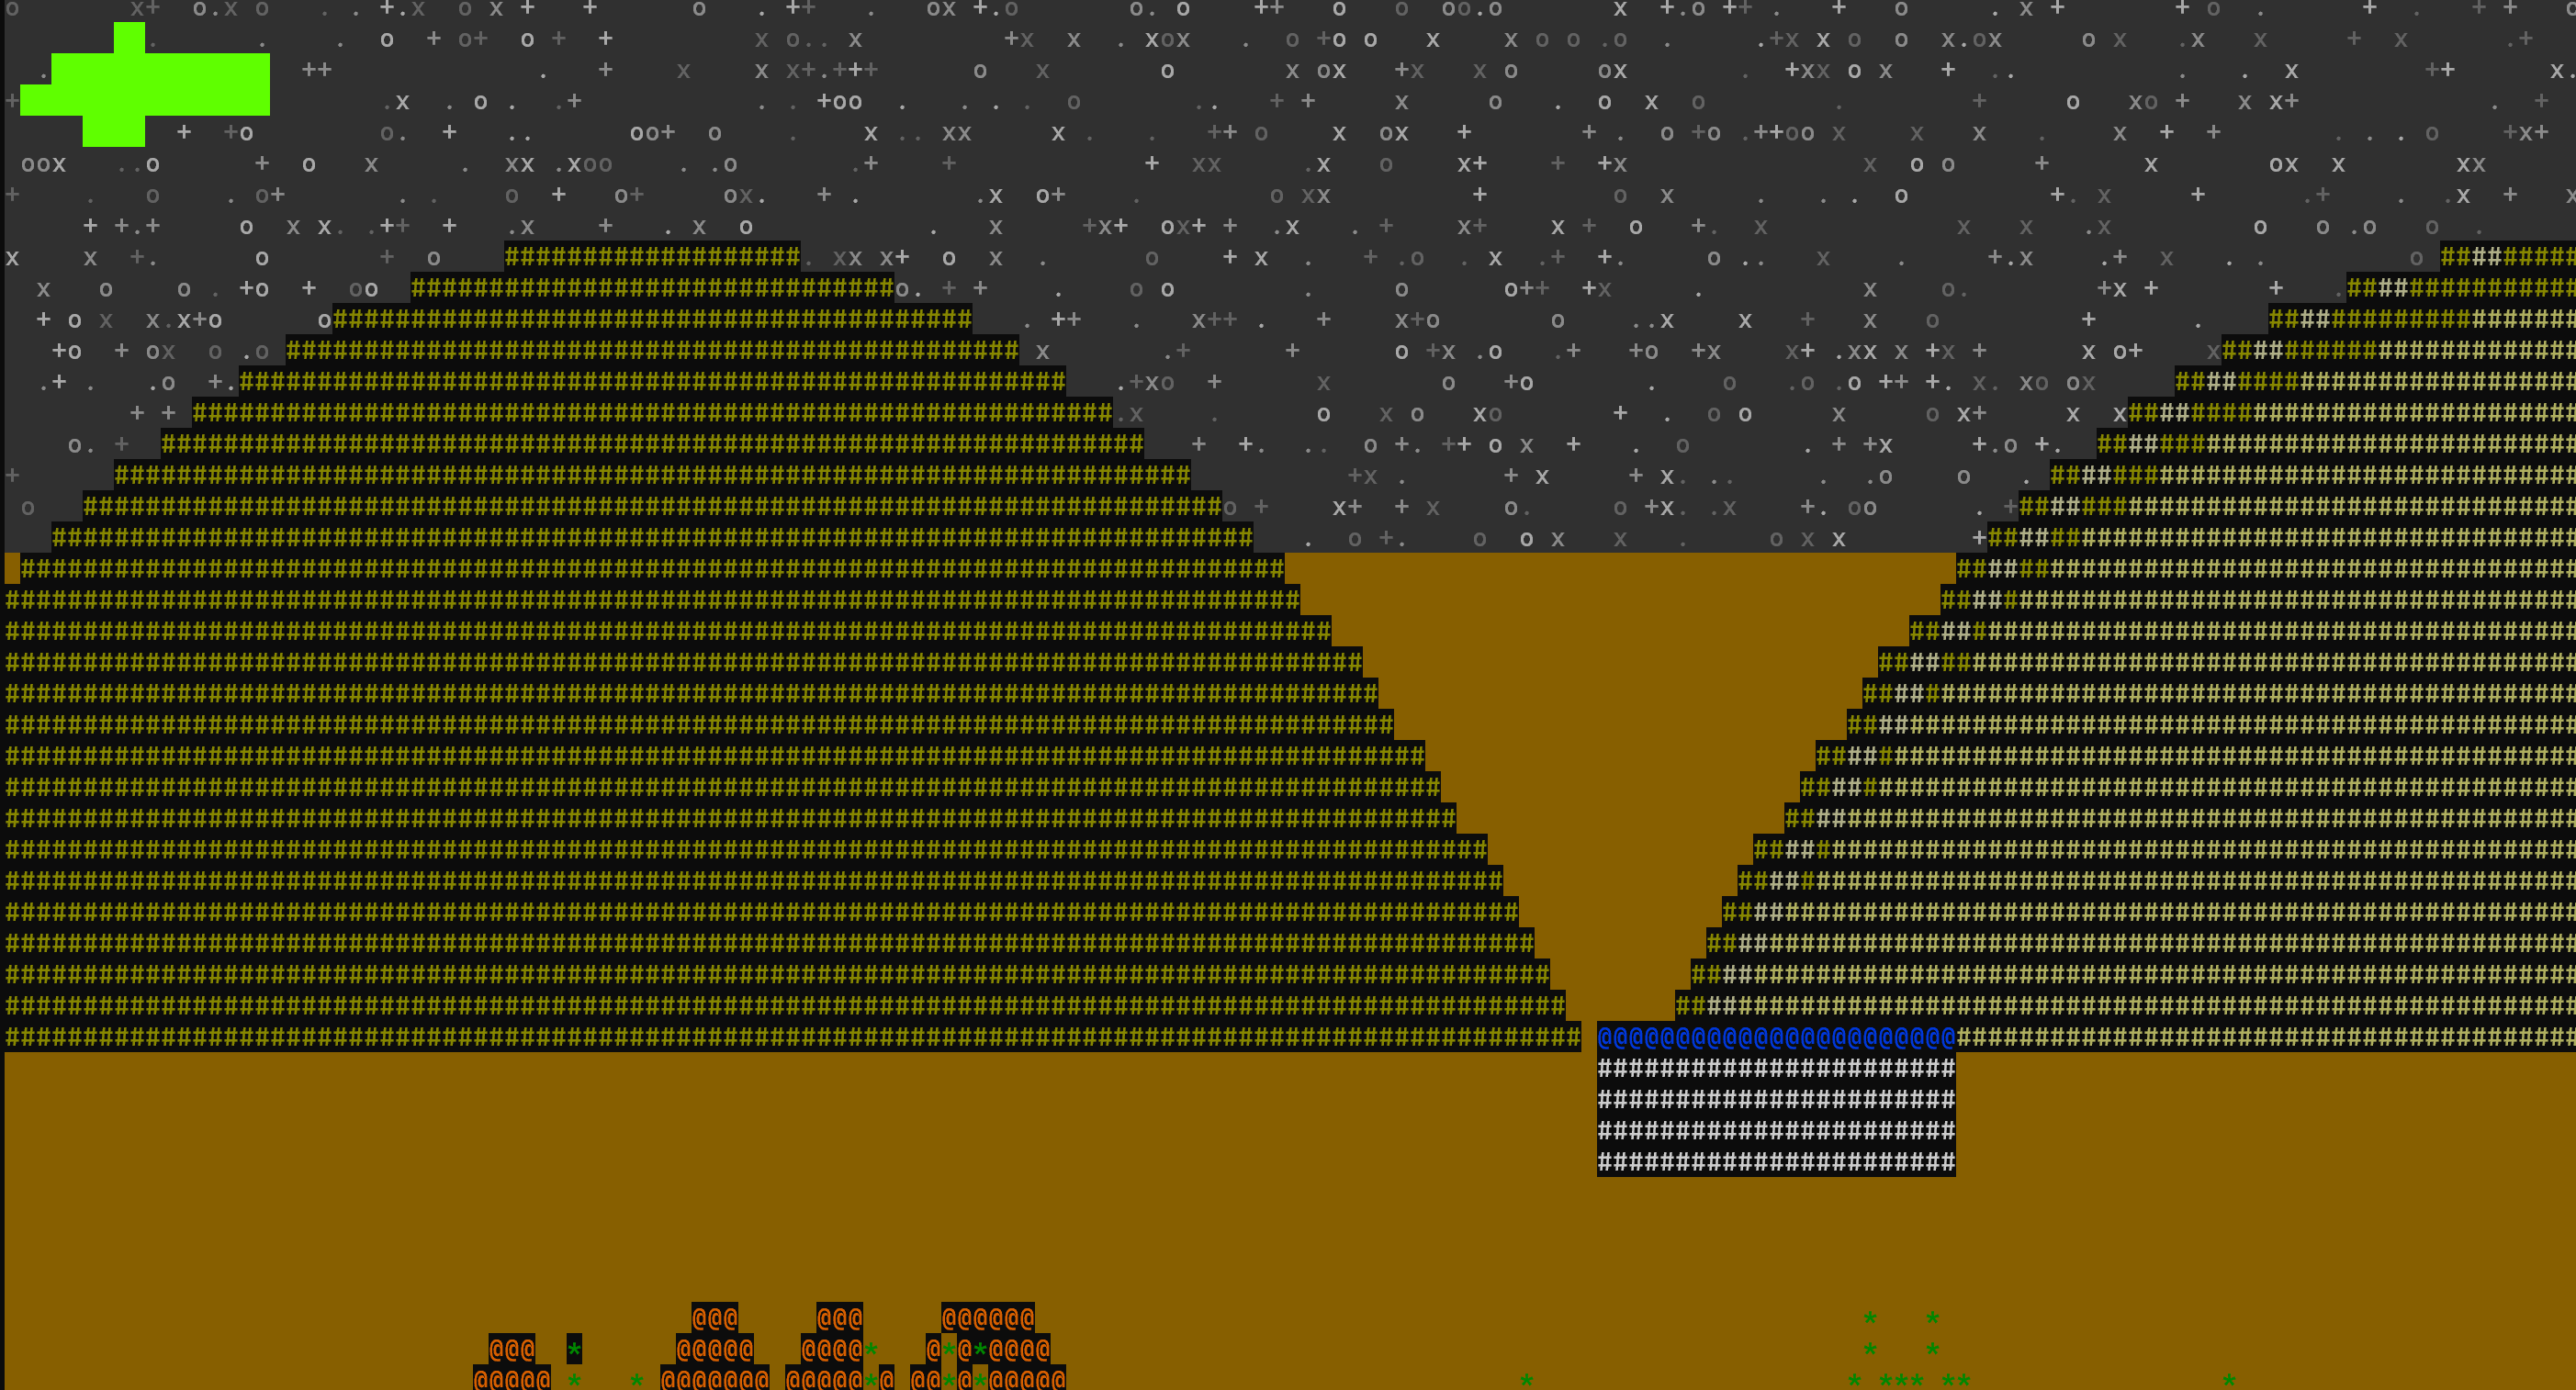
\includegraphics[width=\textwidth]{Screenshot 2025-06-05 105052.png}
    \caption{Bird Mode, note the green arrow in the left}
        
    \end{figure}




\section*{Quick Technical Notes }
This was written using the Rust programming language with use of the console-game-engine package. It also uses the smart pixel filling library I added to this engine, this supports ray-tracing esque coloring.


\section*{Why}
This game came to me as I was writing my keyword project. I think the life and times of Michael K. is one of the more transformative books I have had the privilege of reading. I felt the same way as when I read The Vegetarian (which is very high praise).
K. wants solely to be a gardener so I thought it would be interesting to make a game in which you can do that. I think Michael's hunger is one of the more interesting part of the story and so I struggled to add it to the game. Initially I added a variable \lstinline[language=c]|hunger| so that the game could track the hunger of Michael, and this is how you would lose (death being loss). But as I went on, I thought about how Michael did not seem to get hungry when he was gardening ``Am I to believe that you lived for a year on pumpkin? The human body is not capable of that, Michaels.'' 
I think this is Coetzee's `response' to idea of K. being this ``ethical indian''. By not succumbing to hunger while gardening K. takes the role of a machine, akin to a combine, no longer fully human, simply waiting for his time to harvest. 
I wanted my game to be peaceful and possible to played idly (or even by doing nothing), which is why I added weeds. If you sit long enough the farm will be completely taken over by weeds. The choice as the player is how you want to labor; should you water your crops all the time, you can easily spend all your time watering (this is why I switched the water to being something you fill up), or all your time fighting weeds, or you can plant your seeds and sit passively, waiting for what you planted to be ready to harvest.

Additionally the game supports the idea of the land being something that you have control over, ``The first thing is the land'' So with this game, you are able to control the land as you see fit. 

I also included the birds eye view to support Michaels dream of ``I used to think about flying. I always wanted to fly. I used to stretch out my arms and think I was flying over the fences and between the houses. I flew low over people's heads, but they couldn't see me.'' This was one of my favorite themes of the book. Especially the idea the doctor has where Michael is not eating so that he can ``grow more and more insubstantial till you are all soul and can fly away'' 

Other questions that came to me was one of camps, if I had more time I might have added a system of camps to the game, and my initial idea was too have this, but as I started working and the game progressed into more of Michael's dream than his reality I realized that camps would take away from the dream I was trying to cultivate. 

Another feature I `added' is that I used an unsigned integer to track the `growth' of the crops. Since unsigned integers have a maximum size before they ``roll over'' (its confusing) it means that if you let your plants sit ripe long enough they will return to their juvenile stage. While this was unintentional to start I realized this was apt, since it can be argued that Michael is constantly flitting between being an adult and being a child.

I also used the terminal as the medium for my game because I thought it was interesting to contrast work with gardening. The terminal is where computer scientists do most of our work from, and so it is fitting to make a game where no work exists in a place that is used only for work. 



\end{document}